\documentclass[12pt,a4paper,onecolumn]{article}%{IEEEtran} % altura de letra=10, conferencia, 

\usepackage[utf8]{inputenc}%acentos sin codigo extra \usepackage[utf8]{inputenc}
\usepackage[spanish,es-noshorthands,es-tabla]{babel} %agrega unos caracteres extra al spanish de babel
%%\documentclass[12pt,conference,a4paper,onecolumn]{book}%{IEEEtran} % altura de letra=10, conferencia, formato a4. "`argencon"' o "`IEEEtran"' es la clase del monumento, que si no es el estandar, tiene sus propias opciones, como "`conference"'.journal
%\usepackage[lmargin=2.5cm,rmargin=1.5cm,top=1.5cm,bottom=1.5cm]{geometry} % es para acomodar los margenes
%-------------Configuracion de la UBA
%\documentclass[12pt,a4paper,twoside]{tesis}
% SI NO PENSAS IMPRIMIRLO EN FORMATO LIBRO PODES USAR
%\documentclass[11pt,a4paper]{tesis}
\usepackage[left=2.5cm,right=2cm,bottom=2cm,top=2cm]{geometry}
%-------------Configuracion de la UBA
%\usepackage{mathptmx} % Timer New Roman font
%\renewcommand{\baselinestretch}{1.5} % Interlineado


% Para comentar un codigo rapido es con ctrl+q y para descomendar es con ctrl+w
%\newcommand{\CLASSINPUTbottomtextmargin}{10mm} % redefino el margen inferior
%\usepackage[latin1]{inputenc} %acentos sin codigo extra
%\usepackage[cp1252]{inputenc}% utf8

\usepackage[compress]{cite} %Es para agregar la bibliografia al final
%\usepackage[compress]{natbib} % esta se usa en todos lados. Pero no vale par IEEE
%\usepackage[pdftex]{graphicx} % PDFLaTeX
%\usepackage[dvipdfmx]{graphicx} % PDFLaTeX

%\usepackage[dvips]{graphicx} % LaTeX
%\DeclareGraphicsExtensions{.eps}

\usepackage{graphicx}%es para agregar imagenes 
\usepackage{float} % para que las imagenes entren como flotantes con [H]
%\usepackage[pdftex]{graphicx}%es para agregar imagenes % Tira un error
%\usepackage{subfigure}  %es para las subfiguras
\usepackage{subcaption} % poner mejores subfiguras?
\usepackage{booktabs}
\usepackage[table,xcdraw]{xcolor}
\usepackage{placeins}

%\DeclareGraphicsExtensions{.eps,.png}
%\DeclareGraphicsExtensions{.png,.eps}
%\usepackage[spanish]{babel} % es para castellanizar algunos comandos
%\usepackage[spanish, es-tabla]{babel} % para que en vez de cuadro diga tabla
\usepackage[spanish,es-noshorthands,es-tabla]{babel} %agrega unos caracteres extra al spanish de babel
\usepackage{alltt} %Ver para que es esto, me parece que simplifica el "` vervatim"'
\usepackage{listings} % es para poder cargar los codigos y que se vean bonitos
\renewcommand\lstlistingname{Código} % Sirve para cambiar el titulo de los codigos. En vez de decir "listing"
%\usepackage{eps}  
\usepackage{chngcntr} % para los pies de pagina
\usepackage[hidelinks]{hyperref} % para agregar links "`[hidelinks]"' sirve para sacar el recuadro alrededor del link
\usepackage{amsthm} % ambiente matematico
\usepackage{amsmath} %otro ambiente matematico
\usepackage{amsfonts} % Para agregar las letras de los conjuntos
\usepackage{mathrsfs} % Letras de transformadas
\usepackage{mathtools}%otro ambiente matematico
\usepackage{amssymb} % mas simbolos
%\usepackage{slashbox} % Es para poner la linea en la tabla
\usepackage[compress]{cite} %Es para agregar la bibliografia al final
%\usepackage{hyperref} % para poner un indice con que linkee a todo el texto en el pdf
\usepackage{color} % para poner textos con color 
\usepackage{hyperref} % para poner links
%\usepackage{epsfig} % para poner color en las tablas
\usepackage{multirow}% para poner color en las tablas
\usepackage{colortbl}% para poner color en las tablas. Esta es la mas importante 
%\columncolor[Modelo]{Color}[SepIzq][SepDer] (columnas) \rowcolor[Modelo]{Color}[SepIzq][SepDer] (filas) 
% http://metodos.fam.cie.uva.es/~latex/apuntes/apuntes10.pdf
\usepackage[table]{xcolor}% para poner color en las tablas % http://ctan.org/pkg/xcolor
\usepackage{array} % Para corregir el alineamiento en las tablas
\usepackage{adjustbox} % Para que las tablas no se salgan de los margenes
\usepackage{fancyhdr} % Es para el encabezado y el pie de pagina
\usepackage{stackengine} % darle un espacio a las filas en ambiente tabular
%\hline\xrowht[()]{10pt}
%\usepackage{TeXiS/TeXiS}% Paquete de la plantilla
%\usepackage{blindtext}
\usepackage{enumitem} % Es para cambiar la forma de enumerar:  
% Letras minusculas
%\begin{enumerate}[label=(\alph*)]
% Letras mayusculas
%\begin{enumerate}[label=(\Alph*)]
% Letras romanas
%\begin{enumerate}[label=(\roman*)]
\usepackage{textcomp} % Es para agregar las marcas registradas
% \textregistered\textcopyright
%\sffamily\textregistered\textcopyright
\usepackage{pgfgantt} % Para poner diagramas de gantt
% ------------------- \newcommand
\newcommand{\simulink}{Simulink\textsuperscript{\textregistered}\ }
\newcommand{\matlab}{MATLAB\textsuperscript{\textregistered}\ }
%\renewcommand{\tablename}{Tabla} % para que diga tabla en vez de ``cuadro''
%\newcommand{\be}{\begin{equation}}  %Simplifica la escritura de ecuaciones
%\newcommand{\ee}{\end{equation}}  %Simplifica la escritura de ecuaciones
%\newcommand{\nbe}{\begin{equation*}}  %Simplifica la escritura de ecuaciones
%\newcommand{\nee}{\end{equation*}}  %Simplifica la escritura de ecuaciones
%\newcommand{\m}{\begin{bmatrix}}
%\newcommand{\fm}{\end{bmatrix}}
%\newcommand{\fig}[4]{ % Figuras asi se usa: \fig{Nombrefigura}{epigrafe}{donde? h, t, b, htb}{ancho}
%\begin{figure}[#3]
%\centering
%\includegraphics[width=#4\columnwidth]{./Figuras/#1}
%\caption{#2}\label{fig:#1}
%\end{figure}}
%
%\newcommand{\arr}[2]{ % es para poder apilar ecuaciones NO numeradas
%\begin{equation*}
%\begin{array}{#1} #2 
%\end{array}
%\end{equation*}}
%
%\newcommand{\pap}{paso a paso\  }
%\newcommand{\Mic}{microstepping}
%\newcommand{\xx}{\cellcolor{blue!50}}


% --------------- FIN \newcommand ----------------------
% Para poner un lindo codigo de matlab:
% For faster processing, load Matlab syntax for listings
\definecolor{codegreen}{rgb}{0,0.6,0}
\definecolor{codegray}{rgb}{0.5,0.5,0.5}
\definecolor{codepurple}{rgb}{0.58,0,0.82}
\definecolor{backcolour}{rgb}{0.95,0.95,0.92}
 
\lstdefinestyle{mystyle}{
    backgroundcolor=\color{backcolour},   
    commentstyle=\color{codegreen},
    keywordstyle=\color{magenta},
    numberstyle=\tiny\color{codegray},
    stringstyle=\color{codepurple},
    basicstyle=\ttfamily\footnotesize,
    breakatwhitespace=true,         
    breaklines=true,                 
    captionpos=b,                    
    keepspaces=false,                 
    numbers=left,                    
    numbersep=5pt,                  
    showspaces=false,                
    showstringspaces=false,
    showtabs=false,                  
    tabsize=2
}
 
\lstset{style=mystyle}
  %---------------------------------------------------------
  
  
%Agrego dependencias para el book


%\documentclass[12pt,conference,a4paper,onecolumn]{book}%{IEEEtran} % altura de letra=10, conferencia, formato a4. "`argencon"' o "`IEEEtran"' es la clase del monumento, que si no es el estandar, tiene sus propias opciones, como "`conference"'.journal
%\usepackage[lmargin=2.5cm,rmargin=1.5cm,top=1.5cm,bottom=1.5cm]{geometry} % es para acomodar los margenes
%-------------Configuracion de la UBA
%\documentclass[12pt,a4paper,twoside]{tesis}
% SI NO PENSAS IMPRIMIRLO EN FORMATO LIBRO PODES USAR
%\documentclass[11pt,a4paper]{tesis}
\usepackage[left=2.5cm,right=2cm,bottom=2cm,top=2cm]{geometry}
%-------------Configuracion de la UBA
%\usepackage{mathptmx} % Timer New Roman font
%\renewcommand{\baselinestretch}{1.5} % Interlineado


% Para comentar un codigo rapido es con ctrl+q y para descomendar es con ctrl+w
%\newcommand{\CLASSINPUTbottomtextmargin}{10mm} % redefino el margen inferior
%\usepackage[latin1]{inputenc} %acentos sin codigo extra
%\usepackage[cp1252]{inputenc}% utf8

\usepackage[compress]{cite} %Es para agregar la bibliografia al final
%\usepackage[compress]{natbib} % esta se usa en todos lados. Pero no vale par IEEE
%\usepackage[pdftex]{graphicx} % PDFLaTeX
%\usepackage[dvipdfmx]{graphicx} % PDFLaTeX

%\usepackage[dvips]{graphicx} % LaTeX
%\DeclareGraphicsExtensions{.eps}

\usepackage{graphicx}%es para agregar imagenes 
\usepackage{float} % para que las imagenes entren como flotantes con [H]
%\usepackage[pdftex]{graphicx}%es para agregar imagenes % Tira un error
%\usepackage{subfigure}  %es para las subfiguras
\usepackage{subcaption} % poner mejores subfiguras?
\usepackage{booktabs}
\usepackage[table,xcdraw]{xcolor}
\usepackage{placeins}

%\DeclareGraphicsExtensions{.eps,.png}
%\DeclareGraphicsExtensions{.png,.eps}
%\usepackage[spanish]{babel} % es para castellanizar algunos comandos
%\usepackage[spanish, es-tabla]{babel} % para que en vez de cuadro diga tabla
\usepackage[spanish,es-noshorthands,es-tabla]{babel} %agrega unos caracteres extra al spanish de babel
\usepackage{alltt} %Ver para que es esto, me parece que simplifica el "` vervatim"'
\usepackage{listings} % es para poder cargar los codigos y que se vean bonitos
\renewcommand\lstlistingname{Código} % Sirve para cambiar el titulo de los codigos. En vez de decir "listing"
%\usepackage{eps}  
\usepackage{chngcntr} % para los pies de pagina
\usepackage[hidelinks]{hyperref} % para agregar links "`[hidelinks]"' sirve para sacar el recuadro alrededor del link
\usepackage{amsthm} % ambiente matematico
\usepackage{amsmath} %otro ambiente matematico
\usepackage{amsfonts} % Para agregar las letras de los conjuntos
\usepackage{mathrsfs} % Letras de transformadas
\usepackage{mathtools}%otro ambiente matematico
\usepackage{amssymb} % mas simbolos
%\usepackage{slashbox} % Es para poner la linea en la tabla
\usepackage[compress]{cite} %Es para agregar la bibliografia al final
%\usepackage{hyperref} % para poner un indice con que linkee a todo el texto en el pdf
\usepackage{color} % para poner textos con color 
\usepackage{hyperref} % para poner links
%\usepackage{epsfig} % para poner color en las tablas
\usepackage{multirow}% para poner color en las tablas
\usepackage{colortbl}% para poner color en las tablas. Esta es la mas importante 
%\columncolor[Modelo]{Color}[SepIzq][SepDer] (columnas) \rowcolor[Modelo]{Color}[SepIzq][SepDer] (filas) 
% http://metodos.fam.cie.uva.es/~latex/apuntes/apuntes10.pdf
\usepackage[table]{xcolor}% para poner color en las tablas % http://ctan.org/pkg/xcolor
\usepackage{array} % Para corregir el alineamiento en las tablas
\usepackage{adjustbox} % Para que las tablas no se salgan de los margenes
\usepackage{fancyhdr} % Es para el encabezado y el pie de pagina
\usepackage{stackengine} % darle un espacio a las filas en ambiente tabular
%\hline\xrowht[()]{10pt}
%\usepackage{TeXiS/TeXiS}% Paquete de la plantilla
%\usepackage{blindtext}
\usepackage{enumitem} % Es para cambiar la forma de enumerar:  
% Letras minusculas
%\begin{enumerate}[label=(\alph*)]
% Letras mayusculas
%\begin{enumerate}[label=(\Alph*)]
% Letras romanas
%\begin{enumerate}[label=(\roman*)]
\usepackage{textcomp} % Es para agregar las marcas registradas
% \textregistered\textcopyright
%\sffamily\textregistered\textcopyright
\usepackage{pgfgantt} % Para poner diagramas de gantt
% ------------------- \newcommand
\newcommand{\simulink}{Simulink\textsuperscript{\textregistered}\ }
\newcommand{\matlab}{MATLAB\textsuperscript{\textregistered}\ }
%\renewcommand{\tablename}{Tabla} % para que diga tabla en vez de ``cuadro''
%\newcommand{\be}{\begin{equation}}  %Simplifica la escritura de ecuaciones
%\newcommand{\ee}{\end{equation}}  %Simplifica la escritura de ecuaciones
%\newcommand{\nbe}{\begin{equation*}}  %Simplifica la escritura de ecuaciones
%\newcommand{\nee}{\end{equation*}}  %Simplifica la escritura de ecuaciones
%\newcommand{\m}{\begin{bmatrix}}
%\newcommand{\fm}{\end{bmatrix}}
%\newcommand{\fig}[4]{ % Figuras asi se usa: \fig{Nombrefigura}{epigrafe}{donde? h, t, b, htb}{ancho}
%\begin{figure}[#3]
%\centering
%\includegraphics[width=#4\columnwidth]{./Figuras/#1}
%\caption{#2}\label{fig:#1}
%\end{figure}}
%
%\newcommand{\arr}[2]{ % es para poder apilar ecuaciones NO numeradas
%\begin{equation*}
%\begin{array}{#1} #2 
%\end{array}
%\end{equation*}}
%
%\newcommand{\pap}{paso a paso\  }
%\newcommand{\Mic}{microstepping}
%\newcommand{\xx}{\cellcolor{blue!50}}


% --------------- FIN \newcommand ----------------------
% Para poner un lindo codigo de matlab:
% For faster processing, load Matlab syntax for listings
\definecolor{codegreen}{rgb}{0,0.6,0}
\definecolor{codegray}{rgb}{0.5,0.5,0.5}
\definecolor{codepurple}{rgb}{0.58,0,0.82}
\definecolor{backcolour}{rgb}{0.95,0.95,0.92}
 
\lstdefinestyle{mystyle}{
    backgroundcolor=\color{backcolour},   
    commentstyle=\color{codegreen},
    keywordstyle=\color{magenta},
    numberstyle=\tiny\color{codegray},
    stringstyle=\color{codepurple},
    basicstyle=\ttfamily\footnotesize,
    breakatwhitespace=true,         
    breaklines=true,                 
    captionpos=b,                    
    keepspaces=false,                 
    numbers=left,                    
    numbersep=5pt,                  
    showspaces=false,                
    showstringspaces=false,
    showtabs=false,                  
    tabsize=2
}
 
\lstset{style=mystyle}
  %---------------------------------------------------------
  
  
%Agrego dependencias para el book


\DeclareGraphicsExtensions{.eps,.png}
\author{Sansoni Sebastian}

\newtheorem{definicion}{Definición}[section]
\newtheorem{teorema}{Teorema}[section]
\AtBeginDocument{%
    \LetLtxMacro\oldref{\ref}%
    \DeclareRobustCommand{\ref}[2][]{(\oldref#1{#2})}%
}

%AGREGAR ENCABEZADO con versión, número de tp y la cantidad de hojas puesta así, por ej: 5/12.
%\lhead[\thepage]{. }
\chead[V1.0]{ V1.0}
\rhead[\thepage]{\thepage}

\begin{document}

%\maketitle
\begin{center}
\begin{Large}
Control de trayectoria para un robot móvil de cuatro ruedas en configuración skid-steering  
\end{Large}
\end{center}

\section{Objetivos}
El objetivo general de este trabajo es desarrollar e implementar una librería, basada en sistemas de código abierto, para simular un robot de cuatro ruedas de dirección deslizante con tracción independiente en cada rueda. Esta librería estará enfocada en el desarrollo y testeo de algoritmos de control y planeación de trayectorias para estos tipos de vehículos. 
\subsection{Objetivos Específicos}
\begin{itemize}
\item Implementar un modelo tridimensional dentro del entorno de simulación.
\item Obtener el modelo cinemático el vehículo.
\item Plantear una estrategia de control lineal para hacer seguimiento de trayectorias. 
\item Adquirir el manejo necesario de nuevas herramientas a utilizar.
\item Documentar el trabajo realizado y garantizar que el mismo pueda ser replicable en el futuro.
\end{itemize}
\section{Fundamentos}
A la hora de desarrollar e implementar dispositivos móviles que involucran interacciones con el medio ambiente surgen desafíos imprevistos. Generalmente las aplicaciones que involucran robots, se testean en un entorno controlado, lo cual conlleva a que ese ensayo no represente correctamente el entorno en donde va a desempeñar tareas normalmente. 

Por ejemplo,  cuando se desea testear un algoritmo en un robot móvil, es necesario trasladar el dispositivo al lugar específico de testeo, mantener la carga de las baterías estable durante todo el ensayo, garantizar que las condiciones ambientales sean comunes, entre otras complejidades observadas en el ciclo de desarrollo de un dispositivo que va a operar en ambientes externos.

Otro desafío que aparece normalmente en las conferencias y en los artículos de investigación es que los resultados mostrados son difícilmente replicables, ya sea porque no se cuenta con el dispositivo en si mismo, o porque no está disponible el código y las bases de datos con las cuales se llevó a cabo el ensayo \cite{bon}. 

%Los simuladores han jugado un rol crítico en aplicaciones en donde se involucran robots, ya que son una herramienta rápida y eficiente de testear nuevos conceptos, estrategias y algoritmos.

Muchas de estas dificultades se pueden minimizar incluyendo dentro del ciclo de desarrollo e implementación el uso de simuladores que simulen la dinámica de los cuerpos rígidos en entornos 3D. Estos simuladores, a través de un motor físico  además de resolver las ecuaciones que modelan el problema, incluyen las interacciones con el medio y con otros objetos mediante coeficientes de fricción entre superficies y amortiguamiento viscoso \cite{ode}.

Actualmente existen numerosos software de simulación como  V-REP \cite{vrep}, Gazebo \cite{gazebo}  y Webots \cite{webots}, que incluyen tanto un motor físico, motor gráfico, interacción con sensores, entre otros aspectos que facilitan la simulación de robots y sus sensores en entornos tridimencionales. Siendo los más conocidos  Gazebo y V-REP.  

Por otro lado el Grupo de Investigación en Vehículos y Sistemas Inteligentes (GIVSI) de la Universidad Nacional del Comahue (UNCo) se encuentra desarrollando un vehículo eléctrico de cuatro ruedas fijas con tracción independiente en cada una. El objetivo de este vehículo es que pueda desarrollar tareas dentro de un ambiente agrícola. *[Poner referencias a pip's realizadas, proyectos de investigación, etc.]* Imagenes?

Los robots que tienen cuatro ruedas con dirección deslizante (4WD SSMR , del inglés four wheel drive skid steering mobile robot) % del tipo skid-steering
 son utilizados típicamente como vehículos todo terreno, debido a que se desempeñan satisfactoriamente en superficies de difícil tránsito. En particular esto se debe a una estructura mecánica robusta. Esta ventaja conlleva a que cuando el vehículo cambia su orientación, aparece un deslizamiento lateral entre las ruedas y el suelo . Esto agrega una complejidad el sistema de control ya que se debe tener en cuenta las propiedades dinámicas del sistema \cite{pazderski2004practical}.     


 Es por estos motivos que se propone modelar, identificar e implementar un modelo tridimensional de este vehículo dentro de un entorno de simulación, para luego proponer  estrategias de planeamiento de trayectoria.  
 
%En la literatura hay muchas cosas desarrolladas, sin embargo muy poco en habla hispana. El tema aún está en en desarrollo, ya que hay recientes trabajos que lo introducen como problematica. \cite{snow}. \href{https://youtu.be/FjrgZMmWTNI}{\underline{\color{blue} video}} 
  
\section{Factibilidad}
Al tratarse de un trabajo teórico y de simulación, la factibilidad precipita en la necesidad de una central de computo para correr los algoritmos *[ver como resolver esto]* y el manejo de las tecnologías propias del trabajo. Dentro de los contenidos necesarios se destacan estas materias curriculares:
\begin{itemize}
\item Sistemas de Control.
\item Sistemas controlados por computadora.
\item Procesamiento digital de señales.
\item Técnicas digitales II.
\end{itemize}

Algunos de los temas extracurriculares son:
\begin{itemize}
\item Manejo de lenguajes de programación: python y C++.
\item Uso de control de versiones GIT.
\item Manejo de sistema operativo Linux.
\item Manejo de Gazebo: simulador 3D dinámico especializado en robots.
\item Manejo de la red ROS.
\end{itemize}

Como muchas de estas tecnologías no son el foco principal durante la carrera de grado, se destinará un lapso de tiempo prudente para adquirir el manejo necesario para alcanzar los objetivos propuestos. 

El director de este trabajo se encuentra cursando un doctorado en sistemas de control, es ayudante de primera en la materia sistemas de control en la carrera de electrónica, cuenta con experiencia usando el simulador antes mencionado, modelando e implementando dispositivos móviles  y maneja las otras tecnologías mencionadas previamente *[Cita necesaria RPIC]* . Considerando además que dispone de tiempo para la dirección de este trabajo, esto garantiza de que los objetivos planteados puedan realizarse dentro de los tiempos propuestos. 
\section{Metodología}

\subsection{Actividades específicas}
A continuación se enumeran las actividades propuestas para los objetivos propuestos:

\begin{enumerate}
\item Estudio del modelado cinemático de los robots con configuración SSMR.
\item Estudio e implementación de técnicas de identificación paramétricas enfocado a robots SSMR. 
\item Estudio de diferentes controladores utilizados comúnmente en la bibliografía para robots con configuración SSMR. 
\item Setup de las tecnologías a utilizar. 
\item Modelado dinámico 3D del robot dentro del entorno de simulación en formatos SDF y URDF. Utilizando objetos mallados en formato Collada y STL. 
\item Implementación de dichas estrategias de control en un script  de python version 3 o superior. 
\item Registrar los resultados obtenidos y compararlos con los obtenidos en la bibliografía.
\item Estudio de la tecnología a utilizar.
\item Documentación. 
\item Redacción y escritura del informe final. 
\end{enumerate}
En la figura \ref{fig:gantt} se muestra el diagrama de Gantt  para las actividades propuestas.

\begin{figure}
\centering
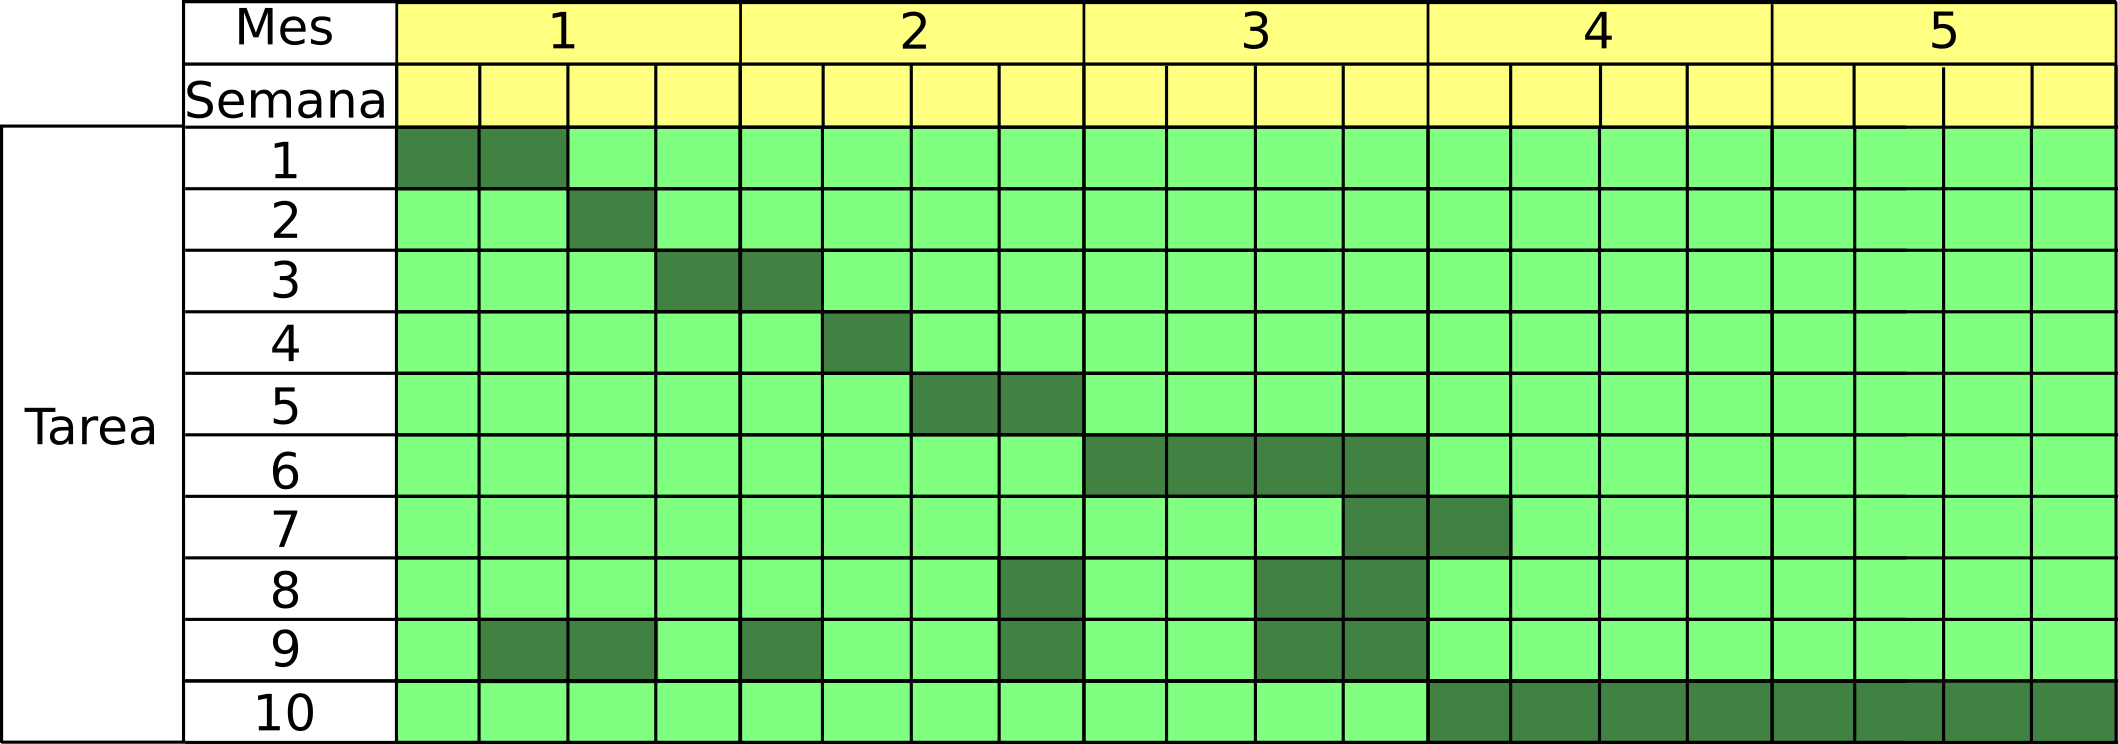
\includegraphics[scale=0.7]{./figuras/gantt.png}
\caption{Diagrama de Gantt propuesto para el trabajo a realizar.}
\label{fig:gantt}
\end{figure}
\section{Bibliografía orientativa}
\bibliographystyle{apalike}%\biboptions{authoryear}
\bibliography{bibliografia}






% OJO!! ##########################################################################3
\end{document}
